\chapter{State-of-the-art} % about 20-30 pages
\chaptermark{State-of-the-art}
\label{chap:sota}
\graphicspath{{./chapters/2-sota/figs/}}

% This thesis work has considered symbol spotting problem as an application of subgraph matching. Symbol spotting has experienced a lot of interests among the graphics recognition community. Here the main task starts by querying a given graphic symbol or model object, usually cropped from a bigger document. The main aim is to search the model object in a target document or set of target documents. In this dissertation we will alternatively name the model object to be queried as \emph{model symbol} or \emph{query symbol} or \emph{pattern} and the corresponding graph representing them as \emph{query graph} or \emph{model graph} or \emph{pattern graph}. And the document or the set of documents where the user intends to find the model symbol as \emph{input document} or \emph{target document} and the corresponding graph as \emph{target graph} or \emph{input graph}. Most of the time the user is interested in getting a ranked list of retrieved zones supposed to contain the queried symbol depending on the similarity or dissimilarity measure. This Chapter contains a review of the state-of-the-art of symbol spotting methods. The major existing research can be classified into five broad families as in~\cite{RusinolThesis2009}, which are listed in Table~\ref{table:sota-ss:relworks}. We review those families as follows:

% \modif{JC:
% Je pense qu'avant t'attaquer avec l'état  de l'art sur les BD, il serait intéressant de faire un état de l'art général sur les méthodes de reconnaissance graphique,  voire les documents non structuré et fond complexes comme évoqué au chp 1.
% De même puisque tu en parles par la suite des méthodes de binarisation (globale, locale, binaire), celles sur les composantes connexes, contour actifs, séparation text/graphique ou clustering?...
% et dire pourquoi ici cela ne marche pas... avant d'enchaîner sur l'état de l'art sur les BD...

% Montrer que tu as une vision plus large du traitement/ analyse des images, des documents graphiques,  des techniques de classification... 

% cela pourrait peut-être se faire  en expliquant la chaine de traitement et détailler rapidement les principales méthodes. 
% }

In this chapter we introduce the document image analysis principles and give an overview of the comics image analysis, holistic understanding of documents and the state-of-the-art applications related to comics in the society.


\section{Document image analysis} % (fold)
\label{sec:document_image_analysis}
Document image analysis is a sub-domain of computer vision systems that includes methods for acquiring, processing, analysing and understanding images in order to produce numerical or symbolic information.
The organization of a document analysis system is highly application dependent. Many functions are specific to the application.
However, there are typical functions which are found in many computer vision systems.

\begin{itemize}
	\item \textbf{Document creation} The first time a document containing a information for humans is transferred to a physical support (e.g. paper sheet, tracing paper, carbon paper, transparent sheet).
	This operation can be performed using various techniques and tools such as plume, pencil, pen, brush, stamp or machine-printed.
	\item \textbf{Image acquisition} A digital image produced by the sensors of various devices (e.g. scanner, camera, web-cam) from the physical document.
	The digital image is an ordered set of pixel with an associated colour value from a certain colour space.
	\item \textbf{Pre-processing} Before a document analysis method can be applied to digitalised image in order to extract some specific piece of information, it is usually necessary to process the image in order to assure that it satisfies certain assumptions implied by the method and its application domain (e.g. noise removal, contrast enhancement, segmentation)~\cite{pal1993review,luccheseyz2001color,bhattacharyya2011brief}.
	\item \textbf{Feature extraction} Feature extraction involves reducing the amount of data accurately.
  Image features are from different levels depending on their distance to pixel information (low level) and human understanding (high level).
	Low level feature such as line, corner, edges and blobs are computed directly from the spatial organisation of pixels~\cite{due1996feature}.
	However, high level information are usually computed from a global view of the image to extract texture and shape for example.
	\item \textbf{Detection/classification} At some point in the processing, decisions are made about which images, point of interests or regions are relevant for further processing.
	\item \textbf{High-level processing} Integration of domain knowledge and making the final decision required for the application.
	This operation may require a user interaction that is sometimes taken into account for future automatic decisions.
\end{itemize}

% An illustration of the application of document analysis system to text recognition and graphics enhancement have been presented by Wong in 1982~\cite{wong1982document} (Figure~\ref{fig:sota:document_analysis_system}).


    %%%%%%%%%%%%%%%%%%%%%%%%%%%%%%%%%%%%%%%%%%%%%%%%%%%%%%%%
    % \begin{figure}[t]%trim=l b r t  width=0.5\textwidth,  
    %   \centering
    %   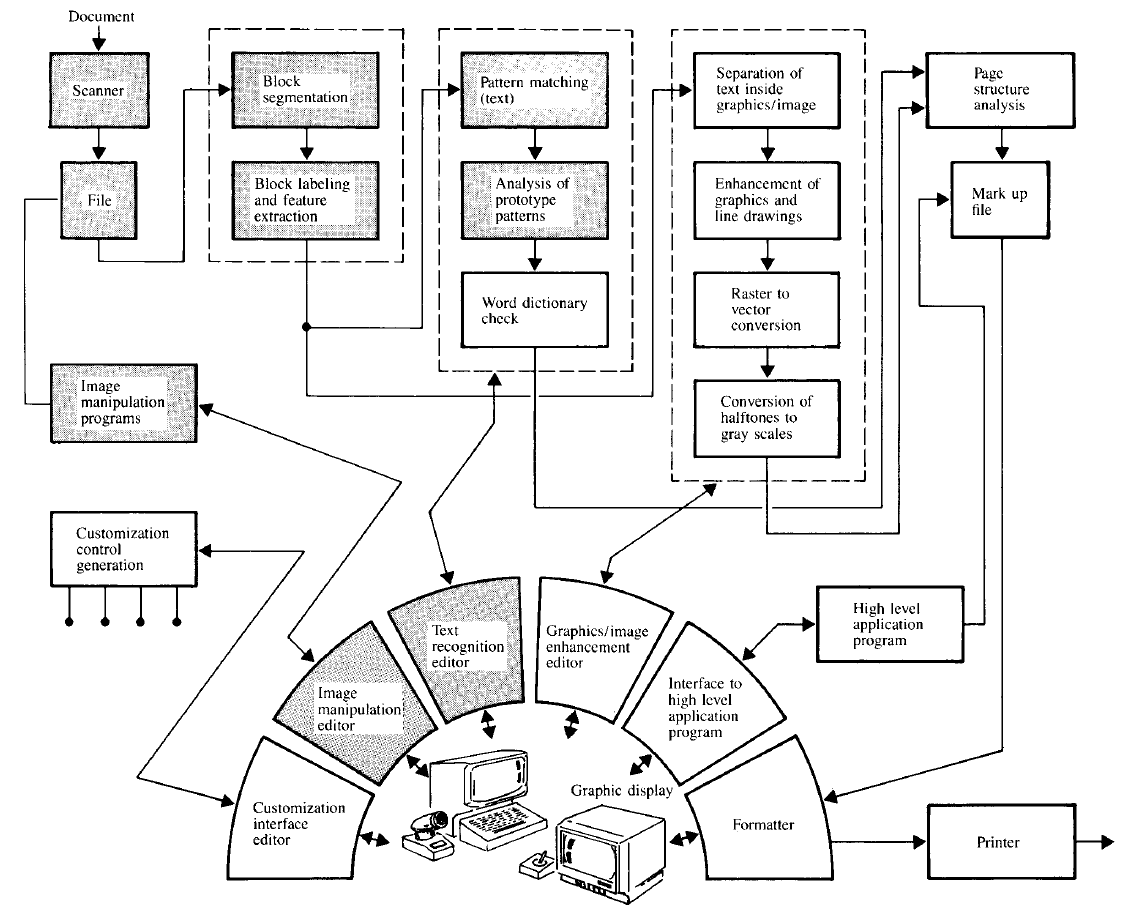
\includegraphics[width=0.9\textwidth]{document_analysis_system.png}
    % \caption[Document analysis system]{Document analysis system~\cite{wong1982document}.}
    % \label{fig:sota:document_analysis_system}
    % \end{figure}
    %%%%%%%%%%%%%%%%%%%%%%%%%%%%%%%%%%%%%%%%%%%%%%%%%%%%%%%%

The content of a document is generally divided into textual and graphical information.
This corresponds to two active research fields, the first one, text recognition aims to convert the text into a character-encoding scheme such as ASCII.
The second one, graphics or symbol recognition, focuses on the recovery of graphical information in documents.
Graphics consist of spatial arrangements of symbols; examples include engineering drawings, maps, architectural drawings, music scores, formulas, tables, charts and some parts of the comic book image content (Figure~\ref{fig:sota:graphics_reco}).

    %%%%%%%%%%%%%%%%%%%%%%%%%%%%%%%%%%%%%%%%%%%%%%%%%%%%%%%%
    \begin{figure}[t]%trim=l b r t  width=0.5\textwidth,  
      \centering
      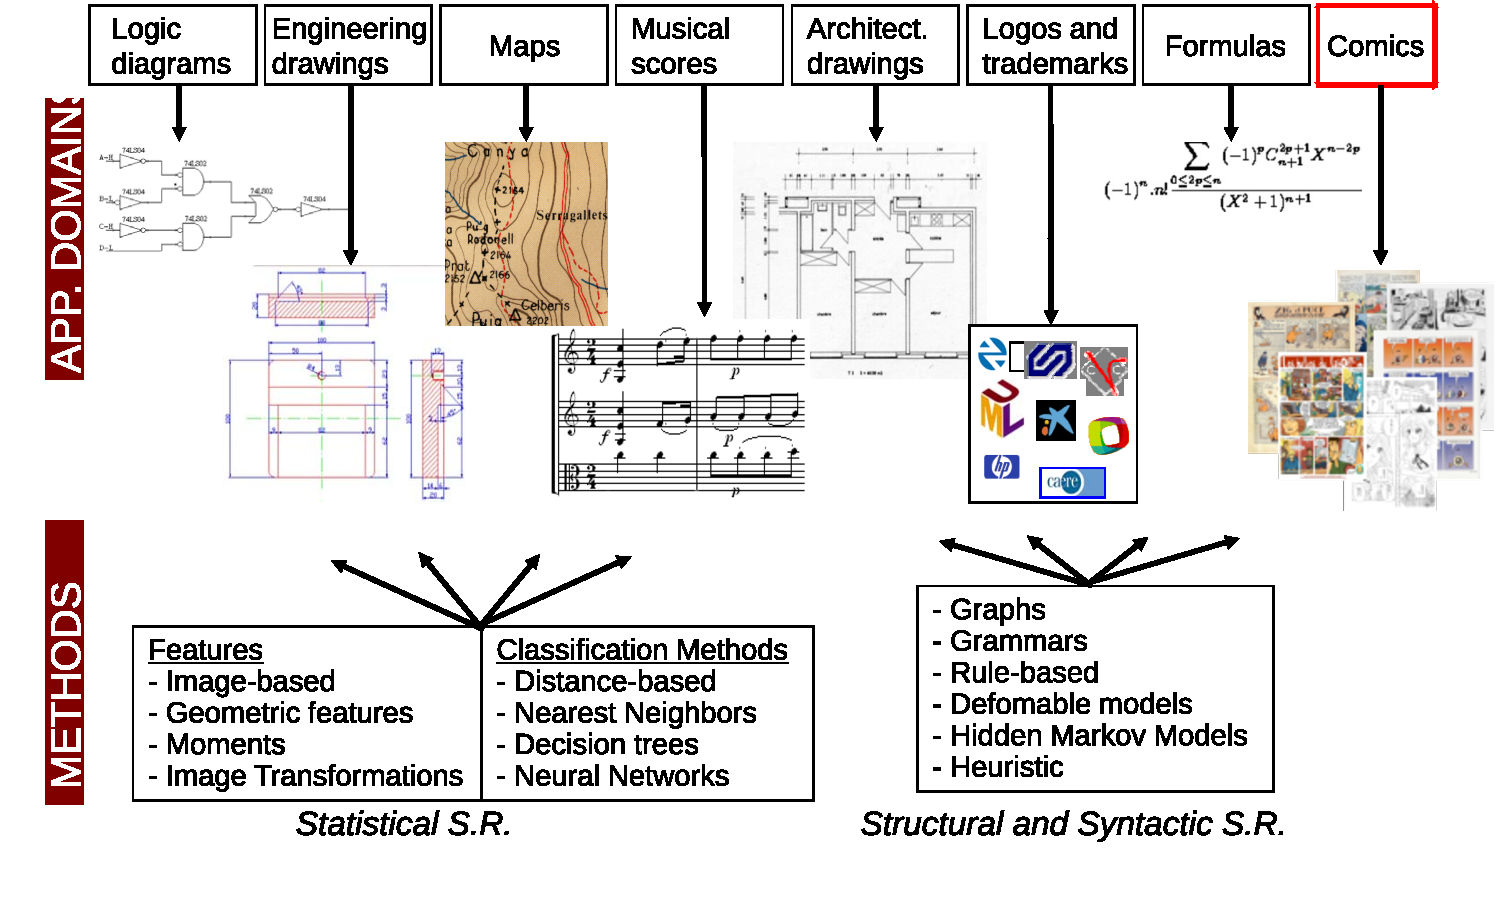
\includegraphics[trim= 15mm 70mm 0mm 0mm, clip, width=0.95\textwidth]{graphics_reco.pdf}
    \caption[Application domains of graphics recognition]{Application domains of graphics recognition.}
    \label{fig:sota:graphics_reco}
    \end{figure}
    %%%%%%%%%%%%%%%%%%%%%%%%%%%%%%%%%%%%%%%%%%%%%%%%%%%%%%%%

Beside its content, a document is usually structured according to its intend of use.
Tang mentioned in 1996 ``A document has two structures: geometric (layout) structure and logical structure.
Extraction of the geometric structure from a document refers to document analysis; mapping the geometric structure into logical structure deals with document understanding''~\cite{tang1996automatic}.
Knowing the structure of the document being processed is always an helpful information that is related to domain knowledge information~\cite{cooperman1998system,breuel2003high}.

Layout analysis consists in segmenting the image into several geometrical blocks that contain the same type of information: text, graphics, table, image, drawing etc.
Then logical information can be retrieved using domain knowledge and the spatial position of the elements (e.g. header and title on the top, page number on the bottom-right corner, reading order).
Layout analysis is not trivial for mixed content documents such as advertisements, posters and comic books.
Those documents use non standard text fonts, size and orientation mixed with graphics, images and logo.% (Figure~\ref{fig:sota:layout_analysis_issues}).

    %%%%%%%%%%%%%%%%%%%%%%%%%%%%%%%%%%%%%%%%%%%%%%%%%%%%%%%%
    % \begin{figure}[t]%trim=l b r t  width=0.5\textwidth,  
    %   \centering
    %   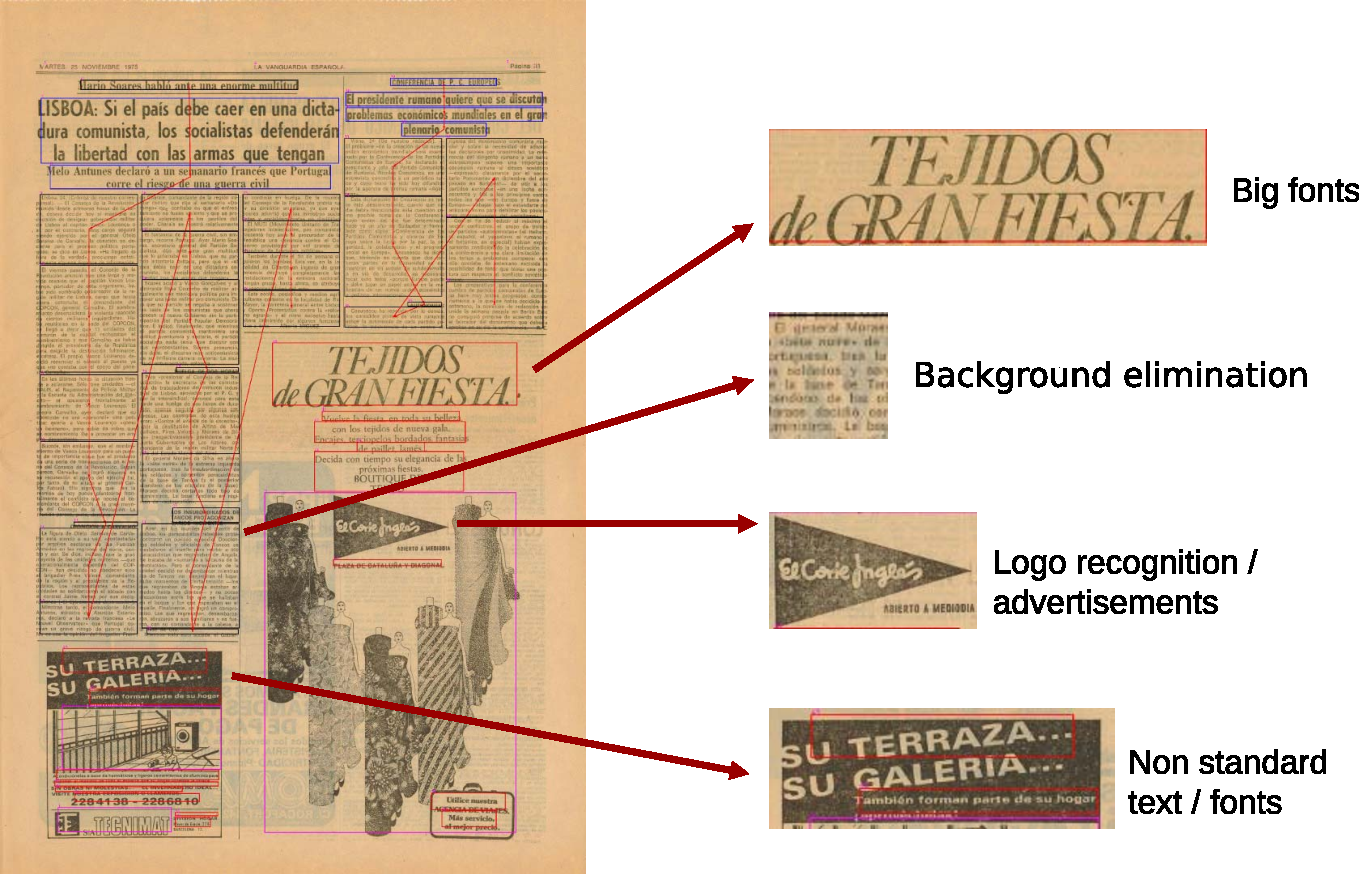
\includegraphics[width=0.8\textwidth]{layout.pdf}
    % \caption[Layout analysis issues]{Layout analysis issues - \emph{Joseph Llados - International Document Image Processing Summer School (IDIPS) 2014}.}
    % \label{fig:sota:layout_analysis_issues}
    % \end{figure}
    %%%%%%%%%%%%%%%%%%%%%%%%%%%%%%%%%%%%%%%%%%%%%%%%%%%%%%%%

Comic book images are composed of text and graphics that can be decomposed as drawings and line drawings.
The diversity of text can be found in comic book images is large.
From speech text which are mostly handwritten to sound effects that are close to drawing sometimes.
Some of the graphics can be assimilated to symbols if we talk about the panels or balloons which have a sort of conventional representation among most of the comic albums.
However, drawings contained in the panel regions do not follow any convention (free art) but contain repeated elements (e.g. comic characters) throughout the album or collection.
This is related to comics art that implies the drawing to be different from others in order to be easily distinguished and recognised by the public.

Comic images are mixed content documents with complex background, especially in the region of panels, that concerns the above mentioned field of research.
Document image analysis being application dependent, we briefly detail the design process of a comic image:

\begin{itemize}
  \item \textbf{Synopsis and scenario} Imagine a story and its decomposition in a sequence of image (storyboard), view angles and format. 
  \item \textbf{Pencil drawing} First rough drawing of the scenario, at this stage, the layout of the page if defined without any details.
  \item \textbf{Inking} The best pencil strokes are inked (permanent) for the final version.
  \item \textbf{Flatting and colouring} Here comes the colours (if any) into all stroke defined regions. Gradient, shadow and other effects are added according to the desired rendering.
  \item \textbf{Lettering and sound effects} Addition of text in reserved areas and sound effects over the graphics at the end.
\end{itemize}

The first challenge of comics book image analysis is to retrieve the layers that corresponds to each step of the comic image design process (e.g. stroke, text, colour).
Processing each layer separately would greatly simplifies layout and content retrieval.
Unfortunately, this decomposition is not obvious because in the final image, the elements are mixed with overlapping and transparency.
Another important issue of document analysis is the noise information added from the creation of the physical document to its digital version.
The main sources of noise are the manual operations variabilities, the degradation over time and the acquisition and storage techniques (Figure~\ref{fig:sota:document_degradation}).


    %%%%%%%%%%%%%%%%%%%%%%%%%%%%%%%%%%%%%%%%%%%%%%%%%%%%%%%%
    \begin{figure}[!ht]%trim=l b r t  width=0.5\textwidth,  
      \centering
      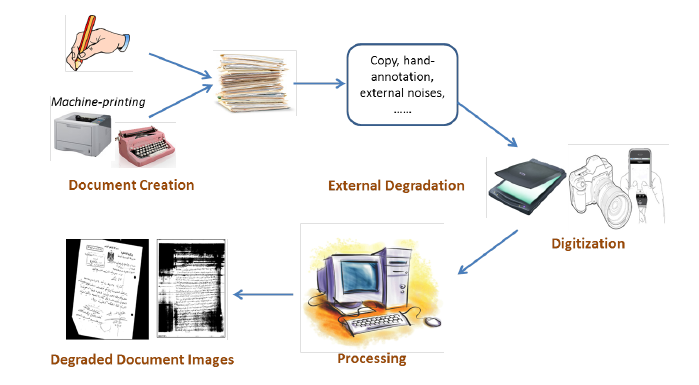
\includegraphics[width=0.85\textwidth]{document_degradation.png}
    \caption[Document degradation sources]{Document degradation sources~\cite{Peng2013Document}.}
    \label{fig:sota:document_degradation}
    \end{figure}
    %%%%%%%%%%%%%%%%%%%%%%%%%%%%%%%%%%%%%%%%%%%%%%%%%%%%%%%%


% Here we briefly detail the most used pre-processing and feature extraction methods related to document image analysis and comics design process.

% \paragraph{Pre-processing} % (fold)
% \label{par:pre_processing}
% Stroke-based images such as comics can be pre-processes is order to extract all the strokes for further analysis.
% Several method from the literature exist, 

% paragraph pre_processing (end)

% \modif{TODO: detail features and classification methods from Figure 2.1?
% Puisque tu en parles par la suite des méthodes de binarisation (globale, locale, binaire), celles sur les composantes connexes, contour actifs, séparation text/graphique ou clustering?



% \begin{itemize}
%   \item Pre-processing methods (\url{http://fr.wikipedia.org/wiki/Segmentation_d'image} FR + EN) -> comic character -> simple PIL with palette + colour L0-smoothing ++
%   \item Feature extraction (textures, outline(), shapes, colour)
%   \begin{itemize}
%     \item Pixel-based (edge, Harris corner, blobs detections)
%     \item Shape-based (thresholding, region growing, connected-component extraction, template matching, Hough transform) 
%     \item Flexible (deformable shapes, active contours)
%   \end{itemize}
%   \item Feature description (to delete?)
%   \begin{itemize}
%     \item Shape-based (compactness, curvature scale space, freeman coding, Fourier transform, invariant moments, texture)
%   \end{itemize}
  
% \end{itemize}
% }



% section document_image_analysis (end)

\section{Comic book image analysis} % (fold)
\label{sec:comic_book_image}

% section comic_book_image (end)

Comics images are mixed content documents combining textual and graphical information to create stories.
Depending on the purpose, the document analysis techniques involved for comics image processing varies a lot between panel, balloon, text and comic character extractions.
The contents of different nature are related to each other to produce a story.
Treating each of the content separately has a limit that can be exceeded in a holistic understanding approach by reaching a higher level of semantic.



\subsection{Panel extraction and layout analysis}
\label{sec:sota:layout_panel}


Panel extraction and ordering have been mainly studied for panel to panel reading.
The need is increasing since the first generation of mobile devices with small screens in colour or B\&W.
In fact, people want to continue reading their favourite comics or manga on the way, without caring kilos of books.
Printed comics require tedious work to be manually scanned and split into screen size parts small enough to avoid zooming and scrolling.

Several techniques have been proposed to automatically extract panels as~\cite{In11}, assuming that panels are small enough elements to be comfortably read on mobile devices.
They are based on white line cutting algorithm~\cite{Duda72,Luyuan2014Automatic,Chan2007Automatic}, recursive X-Y cut~\cite{Han07} or gradient~\cite{Tan07}.
Those methods do not consider empty area~\cite{In11} and border free panels.
These issues have been corrected by connected component approaches~\cite{Arai10} 
%,Rigaud2012LNCS} 
but they are sensible to region that sometimes connect several panels and increase the detection error rate.
Another approach based on growing region and morphological mathematics can remove such connecting elements but also remove information on the panel border~\cite{Ho2012}.
After the region segmentation step, heuristic filtering is often applied to classify panel region according to the size ratio according to the page size, which depends on the page format~\cite{Arai11,Ho2012}.
More recently, new methods have shown interesting results for manga and European comics with different background colours.
They are based on watershed~\cite{ponsard2012ocr}, line segmentation using Canny operator and polygon detection~\cite{Luyuan2014Automatic}, region of interest detection such as corners and line segments~\cite{stommel2012segmentation,Tsai2013Adaptive}.
Panel retargeting have been addressed for manga by Matsui~\cite{Matsui2011}.

Page layout analysis has been studied to calculate the reading order of the panels.
The page layout influences the reader at choosing pathway~\cite{Cohn_2013}, nevertheless few studies~\cite{Guerin2012Ontologies,Ponsard09,Arai2010Automatic} demonstrated the possibility of calculating such Z-path (left-to-right and down) or right-to-left (e.g. Arabic, Japanese) and down~\cite{Li2013Comic,Tsai2013Adaptive} according to the position of the panels. 

%--------------------------------------------------------------------------------
\subsection{Balloon segmentation and tail detection}
\label{sec:sota:balloon_segmentation}

% Balloons or bubbles are the visual unit that conveys dialogue, either spoken or thought
Balloons are a graphic convention used most commonly in comic books, comic strips and cartoons to allow words (and much less often, pictures) to be understood as representing the speech or thoughts of a given character in the comic\footnote{\url{http://en.wikipedia.org/wiki/Speech_balloon}}.
Balloons are developed into a more-or-less oval shape, with a pointer or tail to indicate to which character they belong~\cite{Goggin2010Rise,Varnum2007Language}.
There are many specialized forms of balloons, either traditional or invented~\cite{Marx2006Writing}.
%Balloons or bubbles are key elements in comics, they link graphical and textual elements and are part of the comics style. 

In comics content understanding, speech balloons present a lot of interest since they offer the links between the textual content and the comic characters providing information about the localization of the characters and the tone of speech.
Apart from being crucial for document understanding, balloon detection is also beneficial in applications such as comic character detection~\cite{Sun2011}, content re-targeting~\cite{Matsui2011}, translation assistance and reading order inference~\cite{Guerin2012Ontologies}.

Few works about balloon extraction have been done until now and mainly closed speech balloon have been studied.
Arai~\cite{Arai11} proposed a blob detection method based on connected component detection with four filtering rules applied to manga analysis.
The rules are based on blob minimum size, white pixel occurrence, inclusion of vertical straight lines and width to length ratio (Figure~\ref{fig:Arai_balloon_extraction_process}).
Another connected component approach proposed by Ho~\cite{Ho2012} uses HSV colour space to make a first selection of bright blobs and then consider as balloons the blobs with a ratio between the text area and the blob bounding box higher than sixty percent.


%%%%%%%%%%%%%%%%%%%%%%%%%%%%%%%%%%%%%%%%%%%%%%%%%%%
 \begin{figure}[!ht]  %trim=l b r t  width=0.5\textwidth,
   \centering
  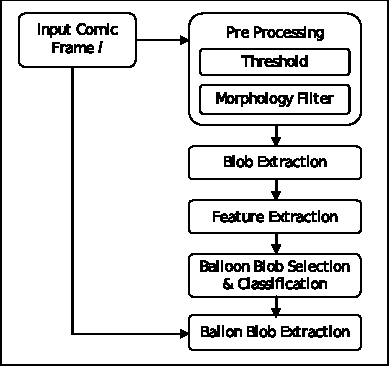
\includegraphics[trim= 0px 0px 0px 0px, clip, width=150px]{Arai_balloon_extraction_process.pdf}
  \caption[Flow diagram of comic balloon detection]{Flow diagram of comic balloon detection using comic blob extraction method proposed by Arai~\cite{Arai11}.}
  \label{fig:Arai_balloon_extraction_process}
 \end{figure}
%%%%%%%%%%%%%%%%%%%%%%%%%%%%%%%%%%%%%%%%%%%%%%%%%%%

The analysis of open balloons with an ``open'' or ``implicit'' contour is quite different than the closed ones which are mainly based on blob analysis and have not been studied before.
In most of the cases, including when contours are implicit, the location of text is generally a good clue to guess where the balloon is.
The problem of speech balloon outline detection can therefore be posed as the fitting of a closed contour around text areas.
The active contour~\cite{Kass1988} model is a deformable model, also known as snake, which tries to minimize an energy associated to the current contour as a sum of an internal and external energy.
Kass~\cite{Kass1988} proposed the original energy functions able to shrink around an object contour, Xu~\cite{Xu1998} proposed the Gradient Vector Flow external force to attract snake from further and handle broken object edges and subjective contours.
% GVF is adapted to our application of non-closed (broken object).
Another extension was proposed by Cohen~\cite{Cohen1991} to make the curve behave like a balloon which is inflated by an additional force.
 %The initial curve needs no longer to be close to the solution to converge''. %We use this last method extension for speech balloon segmentation and customize it in order to detect open balloons.
%Dimos_v1: I don't understand this sentence. multi-resolution contours have been studied to speekd up the multi-resolution model???
Finally, active contour in a multi-resolution context have been studied to speed up the process on multi-resolution image and the multi-resolution model itself~\cite{Leroy1996}.
% We adapt the active contour framework to the domain of comics in~\ch{chap:be}.

% , we propose first approaches in~\ch{chap:be}.
% , balloon contour and tails have not been studied before, we propose first approaches in~\ch{chap:be}.

Balloons provide also an extra information about speech tone according to the different patterns which are along the contour of the balloon.
The shape of the balloon does not provide a lot of information about how the text is spoken, it is more related to the style of the comics and the structure of the panel.
Therefore, we focus on contour classification methods.
In the literature, contour classification is strongly related to shape classification purposes~\cite{sun2005classification,liu1990partial}.
It has been applied for video~\cite{kuhne2001motion,richter2001contour,bader2009}, trademark retrieval~\cite{leung2002trademark}, speech recognition~\cite{grigoriu1994automatic}.
Also, wavelet decomposition~\cite{tieng1997recognition} and invariant moment~\cite{mukundan1998moment}. 
% We propose a first approach in~\ch{chap:be}.

From our knowledge, tail detection have not been studied before, we propose to analyse the contour patterns in order to locate the tail and then perform a local analysis to find its direction (Section~\ref{sec:se:from_balloon_to_tail}).

Balloon classification and tail detection are also important in a context of dialogues and emotions understanding~\cite{millidge2009comic}.



% chapter chap_be (end) ~\ref{sub:be:segmentation}.

%We proposed a first method to extract non closed balloons based on active contours initialized around text areas~\cite{rigaud2013active}, see section~\ref{sub:be:segmentation}.
% This method is able to approximate the contour region, even when it is not printed, based on a domain knowledge which is the mean distance between the balloon contour and the text it contains. 

% A balloon is a spatial container of information that is related to a protagonist using a specific element: the tail.
% The tail is often represented by a discontinuity on contour of the balloon towards the concerned protagonist.
% From our knowledge, there is no work about tail extraction and description in the literature.




\subsection{Text extraction and recognition}
\label{sec:sota:text}

% \begin{itemize}
% 	\item \url{/Text_graphic_separation/2002_Bernhaupt_Using ArtificialNeuralNetwork as image segmentation : application on comics} 
% \end{itemize}

Text localization in real scenes and video frames is an active research topic~\cite{Jung04,ShahabICDAR2011Robust,KaratzasICDAR2013Robust}.
However, applying existing real scene text detection methods to comics would not be optimal to cope with all the different types of text that are combined in comic book documents (e.g. typewritten, handwritten, graphic sound).
If we consider typewritten text, the most similar application to comics is car plate recognition because the text is in a salient and contrasted area with a complex background around the plate such as speech balloon for comics~\cite{anagnostopoulos2008license}.
The documents that have attracted of lot a attention are newspaper, administrative documents, cheques, maps, floor plans and engineering drawings.

Comics differ from classical documents in that they comprise complex backgrounds of a graphical nature. Furthermore, they belong to the class of non-structured documents meaning there is no regular structure present for the prediction of text locations and no layout method applicable.
Comics being unstructured graphical documents, combine the difficulties of both domains, making the task of text localization especially challenging.

Text localization in complex images has been previously studied in scene images~\cite{Weinman09,Epshtein10,Neumann12} and~\cite{Wang10,Meng12}, video sequences~\cite{Wonjun09,Shivakumara09} and digital-born images (Web and email)~\cite{Karatzas07}. 
Text localization in unstructured documents has been studied for teaching boards and slide show presentation~\cite{Oliveira10,Vajda2012Method,Nguyen2013BagOfSubjects}.
However, text localization in documents which are both unstructured and have complex background has received relatively little attention~\cite{Clavelli09}.

% Nevertheless, plates are typewritten with a fixed length.
%From our knowledge, only text localization has been studied, no text segmentation or text recognition yet. This is probably due to the lack of dataset and ground truth to evaluate the algorithms.
Few works concern text extraction in comics, they all rely on speech balloon regions.
Bottom-up approaches use connected component which often relies on the segmentation step~\cite{ponsard2012ocr}.
Su~\cite{Su11} uses Sliding Concentric Windows as text/graphic separation and then apply mathematical morphology and a Support Vector Machine (SVM) classifier to classify text from non-text components. 
%Morphological operations are performed with a fixed mask size, the method is orientation and resolution dependent.
% In~\cite{Rigaud2013VISAPP}, we proposed a adaptive binarisation process based on the Minimum Connected Component Thresholding followed by a text/graphic separation based on contrast ratio and text line grouping, see~\ch{chap:te}.
% Previously, we proposed a k-mean classification of the 
Li~\cite{Li2013Unsupervised} proposed unsupervised speech text localization for comics that trains a Bayesian classifier on aligned connected component and then detect the rest of the text using the classifier for text/non text separation.
 
% Rigaud~\cite{Rigaud12} %~\cite{Rigaud12}
% make use of ``the median value of the border page pixels'' to binarize the image, extract CC and then classify them into ``noise'', ``text'' or ``frame'' (based on CC heights). This method assumes that the page always contains text and that the text background colour is similar to the paper background. 

Top-down approaches starting from balloons (white blobs) detection followed by mathematical morphology operations have been proposed by Arai~\cite{Arai11}, Yamada~\cite{Yam04} and Sundaresan~\cite{Sundaresan2012Text}.
From our knowledge, there are no work concerning graphic sounds (onomatopoeia) and illustrative text extraction.

Text recognition applied to comics is really challenging because it includes most of the difficulties from text recognition in document analysis domain if we consider all the type of text that composed the comics.
From typewritten to handwritten and free-form text in uniform to complex background including image noise, text deformation and overlapping.
Nevertheless, Ponsard~\cite{ponsard2012ocr} solved a sub part of the problem by focusing on speech text of a single font and language for which an OCR system is trained for.


\subsection{Comic character detection}
\label{sec:sota:comic_character}

% \begin{itemize}
	% \item Garfield character detector based on colour histogram \url{/PhD/Biblio_LINK/Object_detection2013_Landry_colour Based Comic Strip Character Recognition.pdf}
	% \item \url{2011_Matsui_Interactive manga retargeting - siggraph11.pdf}
	% \item \url{object/2012_Takayama_FACE DETECTION AND FACE RECOGNITION OF CARTOON CHARACTERS USING FEATURE EXTRACTION}
	% \item \url{object/2007_MASTER_Cheung_Face detection and face recognition of human-like characters in comics}
	% \item Stoke images \url{Object_detection/2010_THESIS_Ta_phuong_inexact_graph_matching_application_to_stroke_images_comics.pdf}
% \end{itemize}


Human detection in computer vision field has been largely studied during the past decades, mainly based on greyscale image and gradients. colour information is rarely relevant for human detection because of clothing and skin colour difference. In videos, moving regions are often used as region of interest.

Although, comics are often a reproduction of human life situations, it is a domain where we can not directly apply human detection based methods.
The main difference is that comic characters (e.g. protagonist, hero) are hand drawn and therefore more variant in terms of deformation, shape and appearance than real life humans (Figure~\ref{fig:sota:tarzan}).
% Comics are composed by a sequence of static snapshots telling a story like a video at a very low frame rate, where we want to detect similar objects. 
In coloured comics, the colour information gives the identity of characters and plays a main role for character spotting with speech balloon positions. 
The simplistic character design allows for easy identification and representation and goes along with how human process visual information~\cite{ahmadimpactsOfManga,medley2010discerningPictures,cohn2010limits}.
%Comics characters are often described using colours while human are described using head feature (e.g. brown hair, blue eyes) because it is the only part that does not change in every day life. 
This is a big difference compared to natural images and human detection, since comics are designed in a way that the information (e.g where are the comic characters, who is talking, where is it going) can be quickly found.% Famous people also use this technique to be easily recognize in video show for example (professional identity).

%%%%%%%%%%%%%%%%%%%%%%%%%%%%%%%%%%%%%%%%%%%%%%%%%%%
 \begin{figure}[!ht]	%trim=l b r t  width=0.5\textwidth,
 	 \centering
 	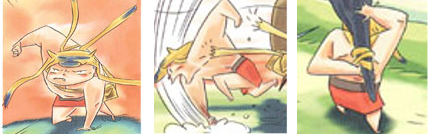
\includegraphics[width=220px]{figs/prunelle.png}
 	\caption[Illustration of the diversity of comics character postures]{Examples of comics character postures. This example shows deformation, pose, rotation, translation and occlusion variations. Image credits: Prunelle, la fille du cyclope, Vicky Portail-Kernel and C\'{e}dric Kernel, Ankama, 2010.
}
 	\label{fig:sota:tarzan}
 \end{figure}
%%%%%%%%%%%%%%%%%%%%%%%%%%%%%%%%%%%%%%%%%%%%%%%%%%%

Recent studies have been published for partial manga copy detection~\cite{Sun2010}, mainly based on shape information because of the absence of colour information.
This work has been extended to Manga copyright infringement protection~\cite{Sun2009Detecting,Sun2013IJDAR} using Maximally Stable Extremal Regions (MSER)~\cite{matas2004robust} or faces~\cite{Viola2004robust} for region detection and Histogram of Oriented Gradients (HOG)~\cite{Dalal05} as region descriptor.
A recent study discuss the local feature extraction and the approximate nearest neighbour (ANN) search~\cite{Iwata2014StudyManga} .
This work shows good results for manga part retrieval which is a subset of the whole comics world.
% In our work we focus on a complementary subset, corresponding to coloured comics analysis.

Coloured comics may be compared to cartoon images sequence, for which a first work based on HOG, SVM and colour attributes has been published in 2012~\cite{Khan12}.
Preliminary work about cartoon and comics faces recognition have been carried out by Kohei~\cite{Kohei2012} and Cheung~\cite{cheung2008face}.
More recently, graph theory has been used to find redundant colour structure in order to automatically localize the most frequent colour group apparition and label them as main characters~\cite{HoGREC2013}.
The thesis of Ta~\cite{TAPhD2010} (section 1.1 and 1.2) gives a good overview about stroke-based image analysis similar to comics, it defines the issues of poor information, occlusion, deformation, inter-class and intra-class variations, scale, spatial and/or temporal relations and structured data.
Ta~\cite{TAPhD2010} also mentions that ``story board scene understanding still remains an open problem, few results are available in the literature about stroke images''.

Another work uses HOG descriptor with redundant information classification to also find the most frequent elements~\cite{SunICDAR2013}.
% It has been improved  
Both graph and descriptor based methods need an image preprocessing step to remove irrelevant redundant elements such as text and speech balloons.

Other interesting approaches try to automatize comic generation~\cite{Tobita2010Comic,WangHYYC12} using image cartoonification and script analysis.

%%%%%%%%%%%%%%%%%%%%%%%%%%%%%%%%%%%%%%%%%%%%%%%%%%%%%%%ù

% Human body and face extractions in real scene image have progressed a lot during the last decades. 
% Nevertheless, the few studies that are related to comics shown that human detection techniques are not appropriate for comics character or need to be trained for specific comic types.
% Those studies concerns the fraud detection in mangas~\cite{Sun2013IJDAR}, cartoon classification~\cite{Khan12} and the detection of the main characters using redundancy information~\cite{SunICDAR2013,HoGREC2013}.
% Preliminary work about cartoon and comics faces recognition have been carried out by Kohei~\cite{Kohei2012} and Cheung~\cite{cheung2008face}.

%We recently proposed~\cite{RigaudDAS2014} a query by example approach that ask the user to select a part of the object he is looking for in one comics image and the system retrieves it automatically everywhere in all the pages of the comics album, assuming that they have been digitized under the same conditions.


\section{Holistic understanding} % (fold)
\label{sec:sota:holistic_understanding}

One of the original goals of image or graphical document analysis was to fully understand the content of any image~\cite{Lamiroy2014Handbook}.
This requires solving several sub-tasks simultaneously, for instance region detection, labelling of meaningful regions and semantic understanding using layout analysis.
In the past, researchers have developed classifiers for tackling each of these sub-tasks independently~\cite{Mao2003Document}.
However, these sub-tasks can help each other.
For instance, in a comics page, if we know the panel positions, then we can make a better guess at the location of the comics characters (they are usually inside the panels).
However, it is not easy to combine different related sub-tasks together.
Previous works concern real scene image analysis~\cite{Blaschke2014Geographic}, retrieval~\cite{Sciascio2011Structured} and understanding~\cite{Li2012Toward,Fidler2012Describing}, medical image annotation using description logic and inference engine~\cite{Hu2003Ontology}, object-based image retrieval~\cite{Mezaris03anontology,Sarwar2013Ontology} (between keyword-based and query-by-example) and image interpretation~\cite{Hudelot2008Fuzzy,Ogier2000Semantic} that mentions the importance of using topological information, distances, directional relative position and much complex relations such as ``between'' and ``surround'' and ``among''.
Also, Geographic Object-Based Image Analysis (GEOBIA)~\cite{Blaschke2014Geographic} makes extensive use of ontologies to interpret maps.

%{\bf ADD} background about document understanding and drawing retrieval (OK: cadastral map).

Recently, comics book images have been also considered.
An ontology of comics has been proposed from a philosophical approach~\cite{Aaron2011}, a semantic annotation tool~\cite{Hermann2012Guided} makes use of previous knowledge and consistency information to suggest new knowledge to the user in a interactive way.
Spatial inferences have been used to infer the comic books reading order, for panel in the page and balloon in the panel~\cite{Guerin2012Ontologies}. 
In~\cite{Sciascio2011Structured}, they highlight the benefit of using contextual information of simple object to build more complex ones.
% From our knowledge, there is no framework for document understanding in the literature that infers new knowledge iteratively and without user interaction (unsupervised).

% section holistic_understanding (end)

\section{Existing applications}
\label{sec:sota:applications}

% \begin{itemize}
	% \item Voice + comic: people tell the comic story and sell them \url{http://vomic.shueisha.co.jp/}
	% \item Comic Chat is a working program, allowing groups of people to communicate over the Internet see \url{2006_Kurlander_Comic_Chat.pdf}
	% \item \url{2010_Tobita_Comic Engine: Interactive System for Creating and Browsing Comic books with Attention Cuing.pdf}
	% \item Comic life: turning your photos into a comic \url{http://plasq.com/}
	% \item Online interactive creation of comics \url{2009_Lopes_Calligraphic Shortcuts for Comics Creation.pdf}

	% \item Software for scripting comics, to define the interactions, time, zoom and region for a kind of video export \url{2012_Raulet_A Sketch-based Interface to Script Comics Reading.pdf}

	% \item Movie to comics: ... the first three factors determine balloon size, and the last factor determines balloon shape ... Emotion can be further exhibited by shape of balloon [1] \url{/PhD/Biblio_LINK/Speech_balloon_analysis/2013_Chu_Optimized Speech Balloon Placement for Automatic_comics_generation.pdf}
% 	\item OCR Manga Reader \url{https://play.google.com/store/apps/details?id=com.cb4960.ocrmr&hl=en}
% 	\item Capture2Text \url{http://capture2text.sourceforge.net/}
% \end{itemize}


Comic books are a graphic art form combining text and images to tell a story.
Comics are now used in a wide variety of styles, not only on paper (e.g., magazines, newspapers, TV show) but also as electronic content (smartphone apps, e-books, websites).
Comics are one of the most popular and familiar forms of graphic content.
People read comics easily and learn many things, so even children can learn about cultures and trends, among other things, through comics even unconsciously.

From this background, we can divide comic-based computer systems into two categories.
One type would be using comics to represent complex information such as online communication in a form of comics~\cite{Kurlander1996} and generating video or story log summaries~\cite{Uchihashi1999Video,Alves2008So,Shamir2006Generating} (computer graphics domain).
Also, it is possible to listen to manga~\cite{Vomic} which have been recorded by people reading the story or to use mobile app for automatic translation~\cite{OCRMangaReader,Capture2Text} (requires user text selection).
These systems are useful to add value to the content while making it more funny and interesting.
The other category concerns the comic design by enabling novices to create comics  interactively using a computer for augmenting an individual user's memory~\cite{SumiSNM2002Comic}, turning photo albums into a comic~\cite{ComicLife3,Chu2013Optimized}, making comic-like video~\cite{Raulet2011Sketch}, making collaborative comics~\cite{Ricardo2009Calligraphic} and exchanging rich message~\cite{Salovaara2007Appropriation}.




\section{Conclusion}
\label{sec:sota:conclusion}


% \begin{itemize}
	% \item Copy/paste from previous publications
	% \item Demonstrate that I understand the topic
	% \item Conclusion and critics

	% \item Navigating comics: an empirical and theoretical approach to strategies of reading comic page layouts \url{2013_Cohn_navigating_comics.pdf}
	% \item 2013 SIGRAPP poster \url{2013_Tsai_Adaptive Manga Re-Layout On Mobile Device.pdf}
% \end{itemize}

Some of the challenges of comics image analysis can be highlighted from the above state-of-the-art reviews.
First, comics image suffer from noise as any other document image processing.
It comes from hardware processes (e.g. drawing techniques, printing and digitization) and software (e.g. image compression).
So efficiently handling noise is crucial for image analysis and understanding.
Knowing the design process of the comics creation helps for image denoising.
Second, according to the results of the reviewed methods, we can order them by level of difficulty, from the simplest to the hardest: panel, balloon, text, comic character and holistic understanding of an image or album.
\modif{add comparison table about genericity, processing time, complexity???}.
Third, most of the works in the literature use different copyrighted images which can not be shared publicly.
Moreover, the authors usually do not share their code.
This is a key issue for researchers which can not share, reproduce and compare results on identical data in a collaborative way.
This is one of the reasons that retains comics analysis to progress as fast as other field of research of document analysis.


In the next chapter, we are going to present a sequential content extraction approach that profits from the relations between elements to guide the retrieval process.
We first process panel and text region extraction followed by speech balloon and tail segmentation.
Then, speech balloon tail indications are used to compute a comic character region of interest according to the spatial organisation of previously extracted elements in the panels.



%the first comics image dataset and ground truth publicly available for researchers. It is a selection of hundred pages from more than twenty different albums from America, Japan and Europe.
% The construction of the dataset and ground truth and a quality assessment test are detailed.
% The hash based technique helps to reduce search space considerably and perform the subgraph matching (symbol spotting) faster.

% The first approach profits from the relations
% between elements to guide the retrieval process. For instance, the panels are first extracted then balloons containing text that are inside panels and finally comic character regions of interest are defined from the speech balloon tail indications.
